\documentclass{beamer}
%
% Choose how your presentation looks.
%
% For more themes, color themes and font themes, see:
% http://deic.uab.es/~iblanes/beamer_gallery/index_by_theme.html
%
\mode<presentation>
{
  \usetheme{default}      % or try Darmstadt, Madrid, Warsaw, ...
  \usecolortheme{crane} % or try albatross, beaver, crane, ...
  \usefonttheme{structureitalicserif}  % or try serif, structurebold, ...
  \setbeamertemplate{navigation symbols}{}
  \setbeamertemplate{caption}[numbered]
} 

\usepackage[english]{babel}
%\usepackage[utf8x]{inputenc}
\usepackage{mathrsfs}

\newtheorem{proposition}{Proposition}
\newtheorem{rem}{Remark}
\newtheorem{goal}{Goal}


\title[Artin Group Presentations]{Artin Group Presentations Arising from Cluster Algebras}
\author{Jacob Haley*, David Hemminger, Aaron Landesman, 
Hailee Peck*}
\institute{University of Minnesota, Twin Cities REU}
\date{\today}


\begin{document}

\begin{frame}
  \titlepage
  \let\thefootnote\relax\footnote{* denotes speaker}
\end{frame}

 
\begin{frame}{Outline}
  \tableofcontents
\end{frame}

\begin{frame}{Brief History}
Fomin and Zelevinsky introduced \textit{cluster algebras}, generated from seed variables. These algebras are of finite type if they are generated from a finite number of seeds. Fomin and Zelevinsky also showed that cluster algebras of finite type can be classified by Dynkin diagrams.
\begin{figure}
\centering
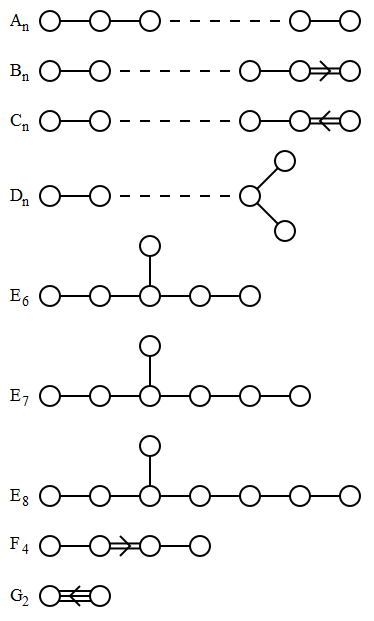
\includegraphics[scale = .25]{dynkindiagrams.PNG}
\caption{Dynkin diagrams}
\end{figure}
\end{frame}

\begin{frame}{Example}
\begin{figure}
\centering
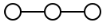
\includegraphics[scale = .65]{DynkinA3.PNG}
\caption{Dynkin diagram of type $A_3$}
\end{figure}

Coxeter group relations:
\begin{itemize}
\item $s_1^2 = s_2^2 = s_3^2 = e$
\item $(s_1s_2)^3 = (s_2s_3)^3 = e$
\item $(s_1s_3)^2 = e$
\end{itemize}

Artin group relations:
\begin{itemize}
\item $\langle s_1, s_2 \rangle ^3 = \langle s_2, s_1 \rangle ^3$
\item $\langle s_2, s_3 \rangle ^3 = \langle s_3, s_2 \rangle ^3$
\item $\langle s_1, s_3 \rangle ^2 = \langle s_3, s_1 \rangle ^2$
\end{itemize}
Alternatively, the above relations correspond to 
\begin{itemize}
\item $s_1s_2s_1 = s_2s_1s_2$
\item $s_2s_3s_2 = s_3s_2s_3$
\item $s_1s_3 = s_3s_1$
\end{itemize}

\end{frame}


\begin{frame}
Barot and Marsh extended the Coxeter group presentations to diagrams of finite type (making an allowance for chordless cycles), and proved that this group presentation is isomorphic to the Coxeter group associated to a Dynkin diagram. They also proved mutation invariance, up to isomorphism, for these Coxeter groups.

\pause
\begin{goal}
Develop variations of relations for the Coxeter group associated to a diagram of finite type provided in Barot-Marsh to define the Artin group $A_{\Gamma}$ corresponding to a diagram $\Gamma$. Prove that for $\Gamma^{\prime} = \mu_k(\Gamma)$, we get $A_{\Gamma} \cong A_{\Gamma^{\prime}}$. 
\end{goal}
\end{frame}

\section{Preliminary Definitions}

\begin{frame}
\begin{definition}
We say a matrix $B$ is \textit{skew-symmetrisable} if there exists a diagonal matrix $D$ of the same size such that $|D_{ii}|>0$ and $DB$ is skew-symmetric.
\end{definition}

\pause

\begin{definition}
A skew-symmetrisable matrix $B$ is \textit{2-finite} if $|B_{ij}B_{ji}| \leq 3$ for all $i, j \in \{ 1, \ldots, n \}$.
\end{definition}

\pause

From the skew-symmetrisable matrix associated to a cluster algebra of finite type, we can associate an diagram $\Gamma$ as follows:\\


For $i, j \in V(\Gamma)$, $i \xrightarrow{w} j$ if and only if $B_{ij}>0$ and $w = |B_{ij}B_{ji}|$ is the weight of the edge.

\end{frame}


\section{Background Results}

\subsection{Mutation Rules}

\begin{frame}{Mutation Rules}
\begin{proposition}
[Proposition 1.4, Barot-Marsh]
Let $B$ be a $2$-finite skew-symmetrisable matrix. Then $\Gamma(\mu_k(B))$ is uniquely determined by $\Gamma(B)$ as follows:
\begin{itemize}
\item Reverse the orientations of all edges in $\Gamma(B)$ incident with $k$ (leaving the weights unchanged)
\item For any path in $\Gamma(B)$ of form $i \xrightarrow{a} k \xrightarrow{b} j$ (i.e. with $a,b$ positive), let $c$ be the weight on the edge $j \rightarrow i$, taken to be zero if there is no such arrow. Let $c'$ be determined by $c'\geq 0$ and 
$c+c' =$ max$(a,b)$. 
Then $\Gamma(B)$ changes in a predetermined way, taking the case $c' = 0$ to mean no arrow between $i$ and $j$.

%%SHOW THE PREDETERMINED WAY ON THE BOARD
\end{itemize}
\end{proposition}

\end{frame}

\begin{frame}{Mutation Rules}
\begin{figure}[h]
\centering
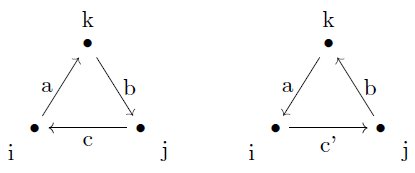
\includegraphics[scale = .65]{mutationrules.PNG}
\caption{Predetermined method for mutation at $k$}
\end{figure}
\end{frame}

\subsection{Chordless cycles underlying $\Gamma$}

\begin{frame}{Unoriented structures underlying $\Gamma$}
\begin{proposition}
[Proposition 2.1, Barot-Marsh]
Any chordless cycle in $\Gamma$ must have an unoriented structure that is one of the following. Furthermore, it must be cyclically oriented.
\begin{figure}[h]
\centering
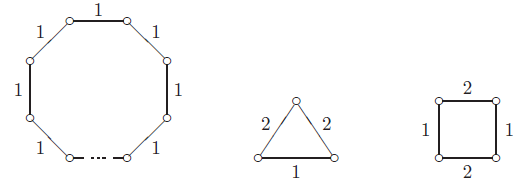
\includegraphics[scale = .65]{chordlesscycles.PNG}
\caption{Possible chordless cycles in a diagram}
\end{figure}

\end{proposition}
\end{frame}


\section{Coxeter group presentation (Barot-Marsh)}

\begin{frame}
\begin{definition}
For a diagram $\Gamma$ and $i, j \in V(\Gamma)$, define 
\begin{displaymath}
m_{ij} = \begin{cases}    2 & \mbox{if } i \mbox{ and } j \mbox{ are not connected;} \\
																	3 & \mbox{if } i \mbox{ and } j \mbox{ are connected by an edge of weight } 1;\\
																	4 & \mbox{if } i \mbox{ and } j \mbox{ are connected by an edge of weight } 2;\\
																	6 & \mbox{if } i \mbox{ and } j \mbox{ are connected by an edge of weight } 3.\\
					\end{cases}
\end{displaymath}	
\end{definition}

This definition will allow us to present generator relations in the group $W_{\Gamma}$.
\end{frame}

\subsection{Generators and Relations}

\begin{frame}

Given a diagram $\Gamma$ of finite type, Barot and Marsh define the Coxeter group $W_{\Gamma}$ with generators $s_i, i = 1,2,\ldots, n$, subject to the following relations:
\begin{block}
   
\begin{itemize}
\item{\alert{(R1)}} $s_i^2 = e$ for all $i$
\item{\alert{(R2)}} $\left(s_is_j\right)^{m_{ij}} = e$ for all $i \neq j$
\end{itemize}

Furthermore, for a chordless cycle $C : i_0 \rightarrow i_1 \rightarrow \cdots \rightarrow i_{d-1} \rightarrow i_0$ and for $a = 0,1,2,\ldots, d-1$, define \textbf{$r\left(i_a, i_{a+1}\right) = s_{i_a}s_{i_{a+1}} \cdots s_{i_{a+d-1}}s_{i_{a+d-2}} \cdots s_{i_{a+1}}$}.\\

\vspace{0.1cm}
Then we have the following relations:
\begin{itemize}
\item{\alert{(R3)(a)}} If all the weights in the edges of $C$ are $1$, then $r(i_a, i_{a+1})^2 = e$
\item{\alert{(R3)(b)}} If $C$ has some edges of weight $2$, then $r(i_a, i_{a+1})^k = e$ where $k = 4-w_a$ and $w_a$ is the weight of the edge $i_a\--\ i_{a-1}$
\end{itemize}
\end{block}
\end{frame}


\subsection{Invariance under Mutation Equivalence}

\begin{frame}
Given a diagram $\Gamma$ and the corresponding Coxeter group $W_{\Gamma}$, Barot and Marsh prove that this group is invariant (up to isomorphism) under mutation of $\Gamma$.

\begin{theorem}
[Theorem 5.4, Barot-Marsh]
\begin{enumerate}
\item Let $\Gamma$ be a diagram of finite type and $\Gamma^{\prime} = \mu_k(\Gamma)$ the mutation of $\Gamma$ at vertex $k$. Then $W_{\Gamma} \cong W_{\Gamma^{\prime}}$.
\item Let $\mathscr{A}$ be a cluster algebra of finite type. Then the groups $W_{\Gamma}$ associated to the diagrams $\Gamma$ arising from the seeds of $\mathscr{A}$ are all isomorphic (to the reflection group associated to the Dynkin diagram associated to $\mathscr{A}$).
\end{enumerate}
\end{theorem}
\end{frame}


\section{Artin group presentation (HHLP)}

\begin{frame}
\begin{block}

Let
\begin{align*}
\langle x_i,x_j \rangle ^k = \begin{cases}
(x_ix_j)^{\frac{k}{2}}, &\text{ if }k \equiv 0 \pmod 2\\
(x_ix_j)^{\frac{k-1}{2}}x_i &\text{ if } k \equiv 1 \pmod 2
\end{cases}
\end{align*}
That is, $\langle x_i,x_j \rangle$ is just an alternating sequence of $x_i$ and $x_j$ of length $k$.  We also write $\langle x_i,x_j\rangle^{-k}$ to denote $\left(\langle x_i,x_j\rangle^k\right)^{-1}$.
\end{block}

\begin{block}

Let $(i_0,\ldots, i_{d-1})$ be an ordered tuple such that the subgraph of $\Gamma$ on the vertices $i_0,\ldots, i_{d-1}$ is a chordless cycle, with edges of nonzero weight from $i_k$ to $i_{k+1}$, where subscripts are taken $\pmod d.$ Then, denote $$p(i_a,i_{a+1}) = s_{i_{a+1}}^{-1}s_{i_{a+2}}^{-1}\dots s_{i_{a-2}}^{-1}s_{i_{a-1}}s_{i_{a-2}}s_{i_{a-3}}\dots s_{i_{a+1}}.$$
\end{block}

\end{frame}
\begin{frame}
Now we have 
\begin{align*}
\langle x_i,x_j \rangle ^k = \begin{cases}
(x_ix_j)^{\frac{k}{2}}, &\text{ if }k \equiv 0 \pmod 2\\
(x_ix_j)^{\frac{k-1}{2}}x_i &\text{ if } k \equiv 1 \pmod 2
\end{cases}
\end{align*}
And $$p(i_a,i_{a+1}) = s_{i_{a+1}}^{-1}s_{i_{a+2}}^{-1}\dots s_{i_{a-2}}^{-1}s_{i_{a-1}}s_{i_{a-2}}s_{i_{a-3}}\dots s_{i_{a+1}}.$$

Additionally, let $$t(i_a,i_{a+1}) = s_{i_a} p(i_a,i_{a+1})  s_{i_a}^{-1}p(i_a,i_{a+1})^{-1}.$$

These definitions will allow us to present generator relations in the group $A_{\Gamma}$.

\end{frame}


\subsection{Generators and Relations}

\begin{frame}
Given a diagram $\Gamma$ of finite type, we define the Artin group $A_{\Gamma}$ with generators $s_i, i = 1,2,\ldots, n$, subject to the following relations (noting that $t(i_a,i_{a+1}) = s_{i_a} p(i_a,i_{a+1})  s_{i_a}^{-1}p(i_a,i_{a+1})^{-1}$):

\begin{block}

\begin{itemize}

\item{\alert{(T2)}} With $m_{ij}$ as defined previously, for all $i \neq j,$ we add the relations
$\langle s_i,s_j \rangle^{m_{ij}}= \langle s_j,s_i \rangle^{m_{ij}}.$

\item{\alert{(T3)}} Let $(i_0,i_1,\ldots,i_{d-1})$ be an ordered tuple as before. If additionally one of the following two conditions hold:
\begin{enumerate}
\item All edges in the chordless cycle are of weight 1 or 2 and the edge $i_{d-1}\rightarrow i_0$ has weight 2.
\item All edges in the chordless cycle have weight $1.$
\end{enumerate}
then we include the relation
$t(i_0,i_1) = e.$

\end{itemize}

\end{block}
\end{frame}

\begin{frame}{Example}
\begin{figure}
\centering
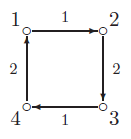
\includegraphics[scale=.5]{4cycle.PNG}
\caption{A 4 cycle with edge weights of 1 and 2}
\end{figure}

\small
Coxeter relations:
\begin{itemize}
\item[R1] $s_1^2 = s_2^2 = s_3^2 = s_4^2 = e$
\item[R2] $(s_1s_2)^3 = (s_3s_4)^3 = e$
\item[R2] $(s_2s_3)^4 = (s_4s_1)^4 = e$
\item[R2] $(s_1s_3)^2 = (s_2s_4)^2 = e$
\item[R3] $r(1,2)^2 = r(3,4)^2 = e$, or $(s_1s_2s_3s_4s_3s_2)^2 = (s_3s_4s_1s_2s_1s_4)^2 = e$
\item[R3] $r(2,3)^3 = r(4,1)^3 = e$, or $(s_2s_3s_4s_1s_4s_3)^3 = (s_4s_1s_2s_3s_2s_1)^3 = e$
\end{itemize}
\end{frame}

\begin{frame}{Example}
\begin{figure}
\centering
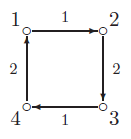
\includegraphics[scale=.5]{4cycle.PNG}
\caption{A 4 cycle with edge weights of 1 and 2}
\end{figure}

\small
Artin relations:
\begin{itemize}
\item[T2] $\langle s_1, s_2 \rangle ^3 = \langle s_2, s_1 \rangle ^3$, or $s_1s_2s_1 = s_2s_1s_2$
\item[T2] $\langle s_2, s_3 \rangle ^4 = \langle s_3, s_2 \rangle ^4$, or $s_2s_3s_2s_3 = s_3s_2s_3s_2$
\item[T2] $\langle s_2, s_4 \rangle ^2 = \langle s_4, s_2 \rangle ^2$, or $s_2s_4 = s_4s_2$
\end{itemize}
The T2 relations $\langle s_3, s_4 \rangle, \langle s_4, s_1 \rangle, \langle s_1, s_3 \rangle$ can be defined in a similar manner.
\begin{itemize}
\item[T3] $t(1,2) = s_1s_2^{-1}s_3^{-1}s_4s_3s_2s_1^{-1}s_2^{-1}s_3^{-1}s_4^{-1}s_3s_2 = e$, or $s_1s_2^{-1}s_3^{-1}s_4s_3s_2 = s_2^{-1}s_3^{-1}s_4s_3s_2s_1$.
\end{itemize}

The T3 relation $t(3,4) = e$ can be defined in a similar manner.
\end{frame}



\begin{frame}
\begin{rem}
Each Artin group has an associated Coxeter group defined by adding in the additional relations $s_i^2 = 1$ for all $i.$ An Artin group is said to be of {\it finite type} if its associated Coxeter group is of finite type. To each Artin group of finite type we can assign it the same Dynkin diagram which is assigned to the Coxeter group associated to the Artin group.
\end{rem}
\end{frame}

\subsection{Invariance under Mutation Equivalence}

\begin{frame}
Given a diagram $\Gamma$ and the corresponding Artin group $A_{\Gamma}$, we prove this group is invariant (up to isomorphism) under mutation of $\Gamma$.

\begin{theorem}
Let $\Gamma$ be a diagram of finite type, and let $\Gamma^{\prime} = \mu_k(\Gamma)$ be the mutation of $\Gamma$ at vertex $k$. Then $A_{\Gamma} \cong A_{\Gamma^{\prime}}$.
\end{theorem}
\end{frame}

\section{Jacob}

\begin{frame}{Unoriented structures underlying $\Gamma$}
\begin{lemma}
[Lemma 2.2, Barot-Marsh]
For $\Gamma$, if we have a subdiagram of $\Gamma$ with three connected vertices, then the unoriented graph underlying the subdiagram must be one of the following:
\begin{figure}[h]
\centering
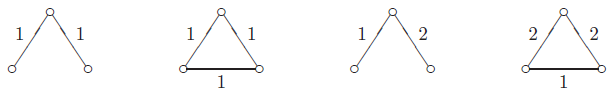
\includegraphics[scale = .65]{3vertconnected.PNG}
\caption{Unoriented 3-vertex connected subdiagrams}
\end{figure}
\end{lemma}

\end{frame}

\subsection{Possible mutations for 3-cycles in $\Gamma$}

\begin{frame}{Possible mutations for $i\--\ k\--\ j$}
\begin{corollary}
[Corollary 2.3, Barot-Marsh]
If in $\Gamma$ we have $i,j,k \in V(\Gamma), i \neq k \neq j$, and we have $i\--\ k\--\ j$, then the only possible mutations for this connected path between the three vertices are the following:
\begin{figure}[h]
\centering
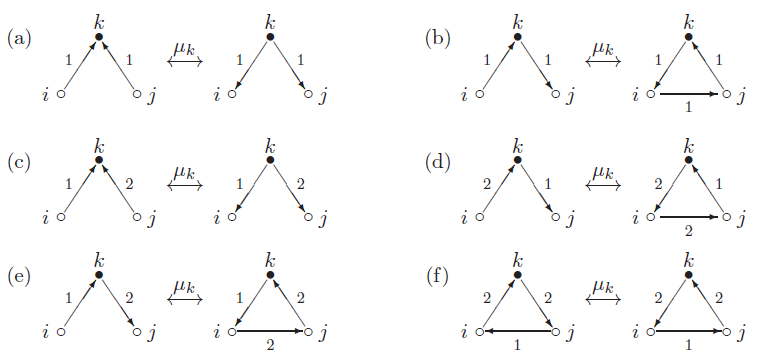
\includegraphics[scale = .40]{mutation3path.PNG}
\caption{Mutation of three connected vertices}
\end{figure}
\end{corollary}
\end{frame}

\begin{frame}
\begin{thebibliography}{69}

\bibitem{BM}[1] Barot, M. and Marsh, R., Reflection Group Presentations Arising from Cluster Algebras, \emph{Preprint}, arXiv:1112.2300 (2011)


\end{thebibliography}

\end{frame}



\end{document}
